%--- Sekcja: Źródła publiczne ---
\section{Źródła publiczne danych}

\begin{frame}{Źródła publiczne - przegląd}
\begin{columns}[c]
    \column{.5\textwidth}
    \begin{alertblock}{Gdzie szukać danych?}
        \begin{itemize}
          \item Media społecznościowe
          \item Fora, blogi, komentarze
          \item Rejestry publiczne
          \item Portale ogłoszeniowe, firmowe
          \item Urządzenia IoT
          \item Narzędzia AI
        \end{itemize}
        \end{alertblock}
    \column{.5\textwidth}
    \centering
    \begin{figure}
        \centering
        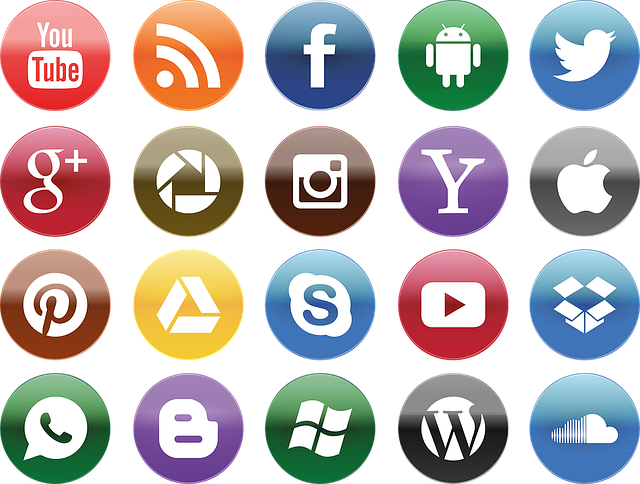
\includegraphics[width=0.75\textwidth]{images/socialMedia.png}
        \label{fig:socialMedia}
    \end{figure}    
\end{columns}
\end{frame}

\begin{frame}{Media społecznościowe}
\begin{block}{}
\begin{itemize}
  \item \textbf{Facebook}: dane osobowe, relacje, lokalizacje z postów
  \item \textbf{X (Twitter)}: tweety, zdjęcia z geolokalizacją
  \item \textbf{LinkedIn}: historia kariery, kontakty, sukcesy
  \item \textbf{Blogi i fora}: styl pisania, emocje, IP, pseudonimy
  \item \textbf{Ustawienia prywatności}: często ignorowane lub błędnie skonfigurowane \cite{zrodlo} \cite{zrodloArtykul}
\end{itemize}
\end{block}
\pause
\begin{exampleblock}{Faktycznie publiczne...}
Wyszukiwarka Google często wystarczy, by dotrzeć do danych „prywatnych”!
\end{exampleblock}
\end{frame}

\begin{frame}{Rejestry i portale firmowe}
\begin{block}{Ogólnodostępne bazy danych}
\begin{itemize}
  \item \textbf{CEIDG}: dane właścicieli firm jednoosobowych
  \item \textbf{KRS}: członkowie zarządu, adresy siedzib
  \item \textbf{CRBR}: beneficjenci rzeczywiści + numery PESEL udziałowców!
  \item \textbf{E-Księgi Wieczyste}: właściciele nieruchomości
  \item \textbf{Portale firmowe, ogłoszenia}: e-maile, telefony, nazwiska \cite{zrodloDzialalnosc}
\end{itemize}
\end{block}
\pause
\begin{alertblock}{Uwaga}
Łącząc kilka baz można zbudować pełny profil osób.
\end{alertblock}
\end{frame}

\begin{frame}{Urządzenia IoT}
\begin{columns}[c]
    \column{.5\textwidth}
    \begin{itemize}
        \item Monitorują obecność domowników
        \item Ustalają rutyny, harmonogramy
        \item Dane wykorzystywane marketingowo, czasem bez zgody!
        \item Przykład: smart lodówka wie, co jesz i kiedy \cite{zrodlo2}
      \end{itemize}
    \column{.5\textwidth}
    \centering
    \begin{figure}
        \centering
        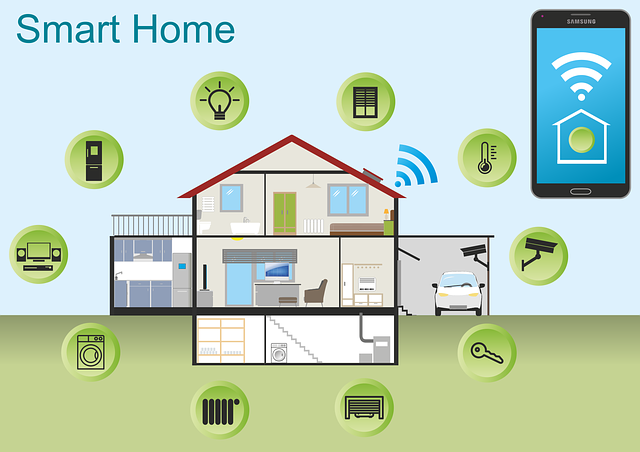
\includegraphics[width=1\textwidth]{images/smart-home.png}
        \label{fig:smart-home}
    \end{figure}    
\end{columns}
\end{frame}

\begin{frame}{Czaty AI jako źródła danych}
\begin{columns}[c]
    \column{.5\textwidth}
    \begin{block}{Zalety... i zagrożenia}
        \begin{itemize}
          \item 43\% pracowników korzysta z AI w pracy
          \item Wiele firm nie kontroluje, co jest wpisywane
          \item AI może zapamiętywać treści zapytań
          \item Analiza stylu, kontekstu, tonu → profilowanie użytkowników \cite{ai}
        \end{itemize}
        \end{block}
    \column{.5\textwidth}
    \centering
    \begin{figure}
        \centering
        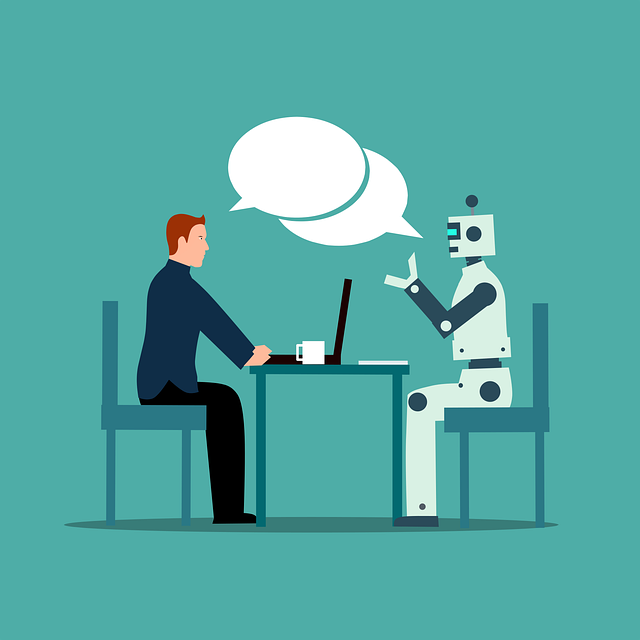
\includegraphics[width=0.75\textwidth]{images/interview.png}
        \label{fig:interview}
    \end{figure}    
\end{columns}
\end{frame}
